\documentclass[11pt,a4paper]{article}
\usepackage[utf8]{vietnam}
\usepackage{amsmath,amssymb}
\usepackage{geometry}
\geometry{top=1.5cm,bottom=1.2cm,left=1.4cm,right=1.4cm,headheight=28pt,headsep=12pt,footskip=18pt}
\usepackage{tikz}
\usepackage{xcolor}
\usepackage{graphicx}
\usepackage{fancyhdr}
\usepackage{tabularx}
\usepackage{enumitem}

\renewcommand{\baselinestretch}{1.06}
\setlength{\parskip}{2pt}
\setlength{\parindent}{0pt}

\definecolor{hfRed}{RGB}{211,47,47}
\definecolor{hfGreen}{RGB}{139,195,144}
\definecolor{myGreen}{RGB}{46,125,50}
\definecolor{myBlue}{RGB}{21,101,192}
\definecolor{mySub}{RGB}{0,105,92}
\definecolor{myPurple}{RGB}{106,27,154}

\pagestyle{fancy}
\fancyhf{}
\fancyhead[L]{\small\itshape\color{hfRed} Tài liệu lưu hành nội bộ}
\fancyhead[R]{\small\itshape\color{hfRed} Thầy \textbf{TRẦN VĂN THẠNH} - 0777.470.803}
\renewcommand{\headrulewidth}{0.8pt}
\renewcommand{\headrule}{\hbox to\headwidth{\color{hfGreen}\leaders\hrule height \headrulewidth\hfill}}

\fancyfoot[L]{\small\itshape\color{hfRed} CS1: 6/15 Nguyễn Hoàng, P. Kim Long, TP Huế \quad|\quad CS2: 24 Đặng Thái Thân, TP Huế}
\fancyfoot[R]{\small\bfseries\color{hfRed} Trang \thepage}
\renewcommand{\footrulewidth}{0.8pt}
\renewcommand{\footrule}{\hbox to\headwidth{\color{hfGreen}\leaders\hrule height \footrulewidth\hfill}}

\begin{document}

% --- HEADER BLOCK ---
\begin{tabularx}{\textwidth}{@{}l X r@{}}
\textbf{\small SỞ GIÁO DỤC VÀ ĐÀO TẠO} & & \textbf{\small ĐỀ THI THỬ GIỮA HỌC KÌ I} \\
\textbf{\normalsize TRƯỜNG THPT CHUYÊN / THPT} & & \textbf{\normalsize MÔN: HÓA HỌC - LỚP 11} \\
\textit{\small (Đề thi gồm có 04 trang)} & & \textit{\small Thời gian làm bài: 45 phút (không kể phát đề)}
\end{tabularx}

\begin{center}
{\color{red!80!black}\textbf{(BẢN GIÁO VIÊN -- CÓ ĐÁP ÁN \& LỜI GIẢI CHI TIẾT)}}\par\vspace{3pt}
\textbf{Họ và tên thí sinh:} \dotfill \quad \textbf{Lớp:} \dots\dots\dots \quad \textbf{Số báo danh:} \dots\dots\dots \hfill \textbf{\large Mã đề 104}
\end{center}
\vspace{-4pt}
{\color{gray!50}\hrule height 0.8pt}
\vspace{6pt}

{\color{myGreen}\bfseries\large PHẦN I (4,5 ĐIỂM). Câu trắc nghiệm nhiều phương án lựa chọn.}

\textit{\small Thí sinh trả lời từ câu 1 đến câu 18. Mỗi câu hỏi thí sinh chỉ chọn một phương án.}
\vspace{3pt}

\textbf{Câu 1.} Ở nhiệt độ cao khoảng 3000 $^\circ\text{C}$, nitrogen trong không khí phản ứng với oxygen tạo thành hợp chất nào sau đây?

\begin{tabularx}{\textwidth}{@{}XXXX@{}}
\textbf{\color{red} A. NO.} & \textbf{B.} NO$_{2}$. & \textbf{C.} NH$_{3}$. & \textbf{D.} N$_{2}$O. \\
\end{tabularx}

\begin{quote}\small
{\color{myBlue}\textbf{$\blacktriangleright$ Lời giải chi tiết:}} Đáp án đúng: \textbf{\color{red} A}\\
Ở nhiệt độ rất cao khoảng 3000 $^\circ\text{C}$ (hoặc khi có tia lửa điện sấm sét), liên kết ba bền vững giữa hai nguyên tử nitrogen (N$\equiv$N) bị bẻ gãy, nitrogen phản ứng với oxygen trong không khí tạo thành nitrogen monoxide:

N$_{2}$(g) + O$_{2}$(g) $\rightleftharpoons$ 2NO(g) (ở khoảng 3000 $^\circ\text{C}$)

Sau đó ở điều kiện thường, khí NO không màu dễ dàng kết hợp tiếp với oxygen tạo NO$_{2}$ màu nâu đỏ (2NO + O$_{2}$ $\longrightarrow$ 2NO$_{2}$).
\end{quote}
\vspace{2pt}

\textbf{Câu 2.} Yếu tố nào sau đây luôn luôn \textit{không} làm dịch chuyển cân bằng của hệ phản ứng?

\begin{tabularx}{\textwidth}{@{}XXXX@{}}
\textbf{A.} Áp suất. & \textbf{B.} Nhiệt độ. & \textbf{\color{red} C. Chất xúc tác.} & \textbf{D.} Nồng độ. \\
\end{tabularx}

\begin{quote}\small
{\color{myBlue}\textbf{$\blacktriangleright$ Lời giải chi tiết:}} Đáp án đúng: \textbf{\color{red} C}\\
Chất xúc tác làm tăng tốc độ của phản ứng thuận và tốc độ của phản ứng nghịch với số lần bằng nhau, do đó chỉ giúp hệ phản ứng nhanh chóng đạt đến trạng thái cân bằng chứ \textit{không làm dịch chuyển cân bằng hóa học} và không làm thay đổi hằng số cân bằng K$_{C}$.
\end{quote}
\vspace{2pt}

\textbf{Câu 3.} Cấu hình electron của nguyên tử nitrogen (Z = 7) là

\begin{tabularx}{\textwidth}{@{}XX@{}}
\textbf{A.} 1s$^{2}$2s$^{3}$2p$^{3}$. & \textbf{\color{red} B. 1s$^{2}$2s$^{2}$2p$^{3}$.} \\
\textbf{C.} 1s$^{2}$2s$^{2}$2p$^{4}$. & \textbf{D.} 1s$^{2}$2s$^{2}$2p$^{5}$. \\
\end{tabularx}

\begin{quote}\small
{\color{myBlue}\textbf{$\blacktriangleright$ Lời giải chi tiết:}} Đáp án đúng: \textbf{\color{red} B}\\
Nguyên tử nitrogen có số hiệu nguyên tử Z = 7. Thứ tự mức năng lượng và sự phân bố electron vào các phân lớp theo đúng quy tắc là: 1s$^{2}$ 2s$^{2}$ 2p$^{3}$. Nguyên tử nitrogen có 2 lớp electron (chu kì 2) và có 5 electron lớp ngoài cùng (nhóm VA).
\end{quote}
\vspace{2pt}

\textbf{Câu 4.} Phản ứng thuận nghịch là phản ứng

\quad \textbf{\color{red} A. phản ứng xảy ra theo hai chiều ngược nhau trong cùng điều kiện.}\\
\quad \textbf{B.} chỉ xảy ra theo một chiều nhất định.\\
\quad \textbf{C.} xảy ra giữa hai chất khí.\\
\quad \textbf{D.} có phương trình hoá học được biểu diễn bằng mũi tên một chiều.\\

\begin{quote}\small
{\color{myBlue}\textbf{$\blacktriangleright$ Lời giải chi tiết:}} Đáp án đúng: \textbf{\color{red} A}\\
Theo định nghĩa SGK Hóa học 11: Phản ứng thuận nghịch là phản ứng hóa học trong đó ở cùng điều kiện, sự chuyển hóa chất phản ứng thành sản phẩm (chiều thuận) và sự chuyển hóa sản phẩm thành chất phản ứng (chiều nghịch) diễn ra đồng thời. Phương trình hóa học của phản ứng thuận nghịch được biểu diễn bằng mũi tên hai chiều ($\rightleftharpoons$).
\end{quote}
\vspace{2pt}

\textbf{Câu 5.} Mưa acid tàn phá nhiều rừng cây, ăn mòn nhiều công trình kiến trúc bằng đá và kim loại. Tác nhân chính tạo ra mưa acid là

\begin{tabularx}{\textwidth}{@{}XXXX@{}}
\textbf{A.} CO$_{2}$. & \textbf{\color{red} B. SO$_{2}$.} & \textbf{C.} H$_{2}$S. & \textbf{D.} CO. \\
\end{tabularx}

\begin{quote}\small
{\color{myBlue}\textbf{$\blacktriangleright$ Lời giải chi tiết:}} Đáp án đúng: \textbf{\color{red} B}\\
Tác nhân chủ yếu gây ra hiện tượng mưa acid là khí sulfur dioxide (SO$_{2}$) và các oxide của nitrogen (NO$_{x}$). Khí SO$_{2}$ bị oxi hóa trong khí quyển với xúc tác ion kim loại hoặc bụi tạo thành SO$_{3}$, sau đó hòa tan vào nước mưa tạo thành sulfuric acid:

2SO$_{2}$ + O$_{2}$ + 2H$_{2}$O $\longrightarrow$ 2H$_{2}$SO$_{4}$.

Do đó, trong các phương án đã cho, SO$_{2}$ là tác nhân chính gây ra mưa acid.
\end{quote}
\vspace{2pt}

\textbf{Câu 6.} Phương trình nào sau đây \textit{không phải} là phương trình phản ứng thuận nghịch?

\begin{tabularx}{\textwidth}{@{}XX@{}}
\textbf{A.} C + CO$_{2}$ $\rightleftharpoons$ 2CO. & \textbf{B.} H$_{2}$ + I$_{2}$ $\rightleftharpoons$ 2HI. \\
\textbf{C.} CaCO$_{3}$ $\rightleftharpoons$ CaO + CO$_{2}$. & \textbf{\color{red} D. NaOH + HCl $\longrightarrow$ NaCl + H$_{2}$O.} \\
\end{tabularx}

\begin{quote}\small
{\color{myBlue}\textbf{$\blacktriangleright$ Lời giải chi tiết:}} Đáp án đúng: \textbf{\color{red} D}\\
Phản ứng trung hòa giữa dung dịch acid mạnh (HCl) và base mạnh (NaOH):

NaOH + HCl $\longrightarrow$ NaCl + H$_{2}$O

là phản ứng một chiều xảy ra hoàn toàn đến cùng, được biểu diễn bằng mũi tên đơn một chiều ($\longrightarrow$). Các phản ứng ở A, B, C đều là các phản ứng thuận nghịch xảy ra trong bình kín.
\end{quote}
\vspace{2pt}

\textbf{Câu 7.} Khi có sấm chớp, trong khí quyển sinh ra chất nào sau đây?

\begin{tabularx}{\textwidth}{@{}XX@{}}
\textbf{A.} Oxide carbon. & \textbf{\color{red} B. Oxide nitrogen.} \\
\textbf{C.} Nước. & \textbf{D.} Không có khí gì sinh ra. \\
\end{tabularx}

\begin{quote}\small
{\color{myBlue}\textbf{$\blacktriangleright$ Lời giải chi tiết:}} Đáp án đúng: \textbf{\color{red} B}\\
Năng lượng cực lớn từ tia chớp tạo nhiệt độ rất cao (hàng nghìn độ C), kích thích phản ứng giữa nitrogen và oxygen trong khí quyển tạo thành nitrogen monoxide: N$_{2}$ + O$_{2}$ $\longrightarrow$ 2NO (oxide nitrogen). Khí NO sau đó tiếp tục phản ứng với oxygen tạo NO$_{2}$, hòa tan vào nước mưa tạo acid nitric HNO$_{3}$ rơi xuống đất cung cấp phân đạm tự nhiên cho cây trồng.
\end{quote}
\vspace{2pt}

\textbf{Câu 8.} Trong công nghiệp, người ta thường điều chế N$_{2}$ từ nguồn nguyên liệu nào sau đây?

\begin{tabularx}{\textwidth}{@{}XXXX@{}}
\textbf{A.} Nitric acid. & \textbf{\color{red} B. Không khí.} & \textbf{C.} Ammonium nitrate. & \textbf{D.} Ammonia. \\
\end{tabularx}

\begin{quote}\small
{\color{myBlue}\textbf{$\blacktriangleright$ Lời giải chi tiết:}} Đáp án đúng: \textbf{\color{red} B}\\
Trong công nghiệp, nitrogen được sản xuất với quy mô lớn bằng phương pháp \textit{chưng cất phân đoạn không khí lỏng}: Không khí sau khi làm sạch bụi, hơi nước và CO$_{2}$ được hóa lỏng dưới áp suất cao và nhiệt độ thấp. Khi nâng dần nhiệt độ của không khí lỏng, khí nitrogen sôi ở -196 $^\circ\text{C}$ bay ra trước và được thu hồi.
\end{quote}
\vspace{2pt}

\textbf{Câu 9.} Hiện tượng phú dưỡng là một biểu hiện của môi trường ao, hồ bị ô nhiễm do dư thừa các chất dinh dưỡng. Sự dư thừa dinh dưỡng chủ yếu do hàm lượng các ion nào sau đây vượt quá mức cho phép?

\begin{tabularx}{\textwidth}{@{}XXXX@{}}
\textbf{A.} Calcium, magnesium. & \textbf{\color{red} B. Nitrate, phosphate.} & \textbf{C.} Sodium, potassium. & \textbf{D.} Chloride, sulfate. \\
\end{tabularx}

\begin{quote}\small
{\color{myBlue}\textbf{$\blacktriangleright$ Lời giải chi tiết:}} Đáp án đúng: \textbf{\color{red} B}\\
Hiện tượng phú dưỡng (eutrophication) xảy ra do nguồn nước mặt tiếp nhận hàm lượng dư thừa các chất dinh dưỡng chứa nguyên tố nitrogen (dưới dạng ion nitrate NO$_{3}^{-}$) và phosphorus (dưới dạng ion phosphate PO$_{4}^{3-}$, HPO$_{4}^{2-}$) từ phân bón nông nghiệp, nước thải sinh hoạt và công nghiệp, kích thích tảo và thực vật thủy sinh bùng phát làm cạn kiệt oxygen hòa tan.
\end{quote}
\vspace{2pt}

\textbf{Câu 10.} Hiện tượng mưa acid được định nghĩa là hiện tượng nước mưa có

\begin{tabularx}{\textwidth}{@{}XX@{}}
\textbf{A.} tính chất sẵn có trong tự nhiên. & \textbf{B.} sự bốc hơi của nước rồi ngưng tụ. \\
\textbf{\color{red} C. giá trị pH < 5,6.} & \textbf{D.} giá trị pH < 7. \\
\end{tabularx}

\begin{quote}\small
{\color{myBlue}\textbf{$\blacktriangleright$ Lời giải chi tiết:}} Đáp án đúng: \textbf{\color{red} C}\\
Nước mưa thông thường hòa tan khí CO$_{2}$ trong khí quyển có pH khoảng 5,6. Khi nước mưa hòa tan thêm các oxide có tính acid mạnh như SO$_{2}$, NO$_{x}$ tạo ra H$_{2}$SO$_{4}$, HNO$_{3}$ làm giá trị pH giảm xuống \textit{dưới 5,6} (pH < 5,6), hiện tượng đó được gọi là hiện tượng \textit{mưa acid}.
\end{quote}
\vspace{2pt}

\textbf{Câu 11.} Bản chất liên kết giữa nguyên tử nitrogen và hydrogen trong phân tử NH$_{3}$ là

\begin{tabularx}{\textwidth}{@{}XX@{}}
\textbf{A.} liên kết hydrogen. & \textbf{\color{red} B. liên kết cộng hoá trị phân cực.} \\
\textbf{C.} liên kết ion. & \textbf{D.} liên kết cộng hoá trị không phân cực. \\
\end{tabularx}

\begin{quote}\small
{\color{myBlue}\textbf{$\blacktriangleright$ Lời giải chi tiết:}} Đáp án đúng: \textbf{\color{red} B}\\
Trong phân tử NH$_{3}$, liên kết giữa nguyên tử N và mỗi nguyên tử H được hình thành do sự dùng chung một cặp electron. Vì độ âm điện của nitrogen (3,04) lớn hơn nhiều so với hydrogen (2,20), cặp electron dùng chung bị hút lệch về phía nguyên tử N, do đó liên kết N-H là \textit{liên kết cộng hóa trị phân cực}.
\end{quote}
\vspace{2pt}

\textbf{Câu 12.} Dạng hình học của phân tử ammonia (NH$_{3}$) là

\begin{tabularx}{\textwidth}{@{}XXXX@{}}
\textbf{A.} hình tứ diện đều. & \textbf{B.} hình tam giác đều. & \textbf{\color{red} C. hình chóp tam giác.} & \textbf{D.} đường thẳng. \\
\end{tabularx}

\begin{quote}\small
{\color{myBlue}\textbf{$\blacktriangleright$ Lời giải chi tiết:}} Đáp án đúng: \textbf{\color{red} C}\\
Nguyên tử N ở trạng thái lai hóa sp$^{3}$, liên kết với 3 nguyên tử H bằng 3 liên kết $\sigma$ và còn lại 1 cặp electron tự do (chưa liên kết). Lực đẩy giữa cặp electron chưa liên kết và các cặp electron liên kết làm các liên kết N-H bị cụp xuống, tạo nên cấu trúc dạng \textit{hình chóp tam giác} (nguyên tử N ở đỉnh chóp, 3 nguyên tử H ở đáy tam giác, góc liên kết H-N-H khoảng 107$^\circ$).
\end{quote}
\vspace{2pt}

\textbf{Câu 13.} Hằng số cân bằng K$_{C}$ của một phản ứng xác định phụ thuộc vào yếu tố nào sau đây?

\begin{tabularx}{\textwidth}{@{}XXXX@{}}
\textbf{A.} Chất xúc tác. & \textbf{\color{red} B. Nhiệt độ.} & \textbf{C.} Áp suất. & \textbf{D.} Nồng độ. \\
\end{tabularx}

\begin{quote}\small
{\color{myBlue}\textbf{$\blacktriangleright$ Lời giải chi tiết:}} Đáp án đúng: \textbf{\color{red} B}\\
Đối với một phản ứng thuận nghịch xác định, hằng số cân bằng K$_{C}$ \textit{chỉ phụ thuộc vào nhiệt độ}. Hằng số K$_{C}$ hoàn toàn không phụ thuộc vào nồng độ ban đầu của các chất, áp suất hay sự có mặt của chất xúc tác.
\end{quote}
\vspace{2pt}

\textbf{Câu 14.} Sulfur được dân gian sử dụng để pha chế vào thuốc trị các bệnh ngoài da. Tên gọi dân gian của sulfur là

\begin{tabularx}{\textwidth}{@{}XXXX@{}}
\textbf{A.} giấm ăn. & \textbf{\color{red} B. diêm sinh.} & \textbf{C.} phèn chua. & \textbf{D.} đá vôi. \\
\end{tabularx}

\begin{quote}\small
{\color{myBlue}\textbf{$\blacktriangleright$ Lời giải chi tiết:}} Đáp án đúng: \textbf{\color{red} B}\\
Trong dân gian từ xa xưa, sulfur (lưu huỳnh) thường được gọi là \textit{diêm sinh} (hoặc lưu hoàng), được sử dụng để điều chế thuốc trị bệnh ngoài da (trị ghẻ, vảy nến), sấy khô chống nấm mốc dược liệu đông y hoặc dùng chế tạo thuốc súng.
\end{quote}
\vspace{2pt}

\textbf{Câu 15.} Phản ứng nào sau đây là phản ứng thuận nghịch?

\quad \textbf{A.} C$_{2}$H$_{5}$OH + 3O$_{2}$ $\longrightarrow$ 2CO$_{2}$ + 3H$_{2}$O.\\
\quad \textbf{B.} Mg + 2HCl $\longrightarrow$ MgCl$_{2}$ + H$_{2}$.\\
\quad \textbf{\color{red} C. 3H$_{2}$ + N$_{2}$ $\rightleftharpoons$ 2NH$_{3}$.}\\
\quad \textbf{D.} 2KClO$_{3}$ $\longrightarrow$ 2KCl + 3O$_{2}$.\\

\begin{quote}\small
{\color{myBlue}\textbf{$\blacktriangleright$ Lời giải chi tiết:}} Đáp án đúng: \textbf{\color{red} C}\\
Phản ứng tổng hợp ammonia từ nitrogen và hydrogen:

N$_{2}$(g) + 3H$_{2}$(g) $\rightleftharpoons$ 2NH$_{3}$(g)

là phản ứng thuận nghịch kinh điển (quá trình Haber - Bosch) diễn ra ở điều kiện nhiệt độ cao, áp suất cao và có chất xúc tác sắt (Fe). Các phản ứng ở A, B, D đều là phản ứng một chiều xảy ra hoàn toàn.
\end{quote}
\vspace{2pt}

\textbf{Câu 16.} Trong công nghiệp, phần lớn lượng sulfur đơn chất sau khi khai thác ở các mỏ được dùng làm nguyên liệu để

\begin{tabularx}{\textwidth}{@{}XX@{}}
\textbf{\color{red} A. sản xuất sulfuric acid.} & \textbf{B.} điều chế thuốc bảo vệ thực vật. \\
\textbf{C.} lưu hoá cao su tự nhiên. & \textbf{D.} bào chế thuốc đông y. \\
\end{tabularx}

\begin{quote}\small
{\color{myBlue}\textbf{$\blacktriangleright$ Lời giải chi tiết:}} Đáp án đúng: \textbf{\color{red} A}\\
Trong nền công nghiệp hóa chất hiện đại, khoảng \textit{90\%} lượng sulfur đơn chất khai thác được sử dụng làm nguyên liệu trực tiếp để \textit{sản xuất sulfuric acid (H$_{2}$SO$_{4}$)} theo phương pháp tiếp xúc; 10\% còn lại dùng để lưu hóa cao su, sản xuất thuốc trừ sâu, phẩm nhuộm, diêm,...
\end{quote}
\vspace{2pt}

\textbf{Câu 17.} Trong phân tử ammonia (NH$_{3}$), nguyên tử nitrogen có số oxi hóa là

\begin{tabularx}{\textwidth}{@{}XXXX@{}}
\textbf{A.} +3. & \textbf{B.} +4. & \textbf{\color{red} C. -3.} & \textbf{D.} +5. \\
\end{tabularx}

\begin{quote}\small
{\color{myBlue}\textbf{$\blacktriangleright$ Lời giải chi tiết:}} Đáp án đúng: \textbf{\color{red} C}\\
Trong hợp chất NH$_{3}$, nguyên tử hydrogen có số oxi hóa +1. Gọi số oxi hóa của nitrogen là x, ta có:

x + 3.(+1) = 0 $\Rightarrow$ x = -3.

Số oxi hóa -3 là số oxi hóa thấp nhất của nitrogen, do đó ammonia chỉ thể hiện tính khử trong các phản ứng oxi hóa - khử.
\end{quote}
\vspace{2pt}

\textbf{Câu 18.} Các yếu tố có thể ảnh hưởng đến sự chuyển dịch cân bằng hoá học là

\begin{tabularx}{\textwidth}{@{}XX@{}}
\textbf{A.} nồng độ, áp suất và diện tích bề mặt. & \textbf{\color{red} B. nồng độ, nhiệt độ và áp suất.} \\
\textbf{C.} áp suất, nhiệt độ và chất xúc tác. & \textbf{D.} nồng độ, nhiệt độ và chất xúc tác. \\
\end{tabularx}

\begin{quote}\small
{\color{myBlue}\textbf{$\blacktriangleright$ Lời giải chi tiết:}} Đáp án đúng: \textbf{\color{red} B}\\
Theo nguyên lí Le Chatelier, các yếu tố làm chuyển dịch cân bằng hóa học gồm có: \textit{nồng độ, nhiệt độ và áp suất} (đối với phản ứng có chất khí và có sự biến thiên tổng số mol khí). Chất xúc tác và diện tích bề mặt chất rắn chỉ ảnh hưởng đến tốc độ phản ứng chứ không làm chuyển dịch vị trí cân bằng.
\end{quote}
\vspace{2pt}

\vspace{6pt}
{\color{myGreen}\bfseries\large PHẦN II (4,0 ĐIỂM). Câu trắc nghiệm đúng sai.}

\textit{\small Thí sinh trả lời từ câu 1 đến câu 4. Trong mỗi ý a), b), c), d) ở mỗi câu, thí sinh chọn đúng hoặc sai.}
\vspace{3pt}

\textbf{Câu 1.} Khí NO$_{x}$ là một trong các nguyên nhân gây nên hiện tượng mưa acid, sương mù quang hóa, hiện tượng phú dưỡng,… làm ô nhiễm môi trường nghiêm trọng.

\begin{center}
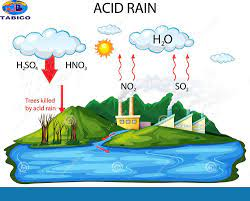
\includegraphics[width=0.42\textwidth]{images_hoa11_de04/acid_rain.png}
\end{center}
\textbf{a)} [\textbf{\color{red} ĐÚNG}] Hoạt động giao thông vận tải làm phát sinh NO$_{x}$.\\
\textbf{b)} [\textbf{\color{red} ĐÚNG}] Hoạt động của nhà máy nhiệt điện làm phát sinh NO$_{x}$.\\
\textbf{c)} [\textbf{\color{red} ĐÚNG}] Hoạt động của núi lửa làm phát sinh NO$_{x}$.\\
\textbf{d)} [\textbf{\color{red} ĐÚNG}] Hoạt động đốt nhiên liệu hóa thạch làm phát sinh NO$_{x}$.\\

\begin{quote}\small
{\color{myBlue}\textbf{$\blacktriangleright$ Giải thích chi tiết:}}\\
- Ý a) \textbf{ĐÚNG}: Động cơ đốt trong của các phương tiện giao thông (ô tô, xe máy, máy bay) vận hành ở nhiệt độ và áp suất cao làm N$_{2}$ và O$_{2}$ trong không khí phản ứng tạo thành NO, sau đó thoát ra môi trường hóa nâu thành NO$_{2}$.

- Ý b) \textbf{ĐÚNG}: Nhà máy nhiệt điện đốt cháy nhiên liệu than đá hoặc khí đốt ở nhiệt độ cao sinh ra lượng lớn NO$_{x}$ cùng với SO$_{2}$.

- Ý c) \textbf{ĐÚNG}: Hoạt động phun trào của núi lửa với nhiệt độ macma cực lớn trên 1000 $^\circ\text{C}$ kích hoạt phản ứng giữa N$_{2}$ và O$_{2}$ trong khí quyển, đồng thời giải phóng các chất chứa nitrogen từ sâu trong vỏ Trái Đất, sinh ra NO$_{x}$ tự nhiên.

- Ý d) \textbf{ĐÚNG}: Việc đốt nhiên liệu hóa thạch (than đá, dầu mỏ, khí thiên nhiên) trong các ngành công nghiệp và sinh hoạt là nguồn nhân tạo chủ yếu phát thải NO$_{x}$ vào bầu khí quyển.
\end{quote}
\vspace{2pt}

\textbf{Câu 2.} Cho các phát biểu sau về nguyên tố nitrogen (N, Z = 7):

\textbf{a)} [\textbf{\color{mySub} SAI}] Nguyên tố nitrogen thuộc chu kì 3, nhóm VA trong bảng tuần hoàn.\\
\textbf{b)} [\textbf{\color{red} ĐÚNG}] Trong một số hợp chất, nguyên tử nitrogen có thể dùng cặp electron hoá trị riêng để tạo một liên kết cho – nhận với nguyên tử khác.\\
\textbf{c)} [\textbf{\color{red} ĐÚNG}] Nguyên tử nguyên tố nitrogen có cấu hình electron là 1s$^{2}$2s$^{2}$2p$^{3}$.\\
\textbf{d)} [\textbf{\color{mySub} SAI}] Nguyên tử nguyên tố nitrogen có 3 electron hoá trị.\\

\begin{quote}\small
{\color{myBlue}\textbf{$\blacktriangleright$ Giải thích chi tiết:}}\\
- Ý a) \textbf{SAI}: Nitrogen (Z = 7) có cấu hình electron là 1s$^{2}$2s$^{2}$2p$^{3}$, có 2 lớp electron nên thuộc \textbf{chu kì 2} (không phải chu kì 3), nhóm VA.

- Ý b) \textbf{ĐÚNG}: Ở lớp vỏ ngoài cùng, nguyên tử nitrogen có 1 cặp electron tự do (chưa liên kết). Trong các phân tử như NH$_{3}$, nitrogen có thể dùng cặp electron này để tạo liên kết cho - nhận với ion H$^{+}$ tạo cation ammonium (NH$_{4}^{+}$).

- Ý c) \textbf{ĐÚNG}: Với số hiệu Z = 7, cấu hình electron chuẩn là 1s$^{2}$2s$^{2}$2p$^{3}$.

- Ý d) \textbf{SAI}: Lớp ngoài cùng (n = 2) của nitrogen có 2 + 3 = 5 electron, do đó nitrogen có \textbf{5 electron hóa trị} (chứ không phải 3; 3 là số electron độc thân ở phân lớp 2p).
\end{quote}
\vspace{2pt}

\textbf{Câu 3.} Hydrogen chloride phân li trong nước theo phương trình sau: HCl $\longrightarrow$ H$^{+}$ + Cl$^{-}$

\textbf{a)} [\textbf{\color{red} ĐÚNG}] Theo thuyết Bronsted – Lowry về acid – base thì HCl là acid.\\
\textbf{b)} [\textbf{\color{mySub} SAI}] Khi hòa tan trong nước, chỉ một phần các phân tử HCl bị phân li thành ion.\\
\textbf{c)} [\textbf{\color{red} ĐÚNG}] HCl là chất điện li mạnh.\\
\textbf{d)} [\textbf{\color{red} ĐÚNG}] Khi hòa tan trong nước, toàn bộ các phân tử HCl đều bị phân li thành ion.\\

\begin{quote}\small
{\color{myBlue}\textbf{$\blacktriangleright$ Giải thích chi tiết:}}\\
- Ý a) \textbf{ĐÚNG}: Theo thuyết Brønsted – Lowry, acid là chất cho proton (H$^{+}$). Trong dung dịch nước: HCl + H$_{2}$O $\longrightarrow$ H$_{3}$O$^{+}$ + Cl$^{-}$, phân tử HCl nhường H$^{+}$ cho H$_{2}$O nên HCl là acid.

- Ý b) \textbf{SAI}: HCl là chất điện li mạnh, khi tan trong nước phân li hoàn toàn thành ion, không phải "chỉ một phần".

- Ý c) \textbf{ĐÚNG}: HCl là acid mạnh và là chất điện li mạnh điển hình.

- Ý d) \textbf{ĐÚNG}: Đây là định nghĩa chất điện li mạnh: khi tan trong nước, toàn bộ các phân tử hòa tan đều phân li hoàn toàn thành ion.
\end{quote}
\vspace{2pt}

\textbf{Câu 4.} Cho các phát biểu sau về đặc điểm của phản ứng thuận nghịch:

\textbf{a)} [\textbf{\color{red} ĐÚNG}] Trong hệ phản ứng thuận nghịch luôn tồn tại đồng thời chất sản phẩm và chất tham gia.\\
\textbf{b)} [\textbf{\color{mySub} SAI}] Khi phản ứng thuận nghịch đạt trạng thái cân bằng hóa học, phản ứng dừng lại.\\
\textbf{c)} [\textbf{\color{red} ĐÚNG}] Chỉ có phản ứng thuận nghịch mới đạt đến trạng thái cân bằng hóa học.\\
\textbf{d)} [\textbf{\color{red} ĐÚNG}] Hiệu suất của phản ứng thuận nghịch luôn nhỏ hơn 100\%.\\

\begin{quote}\small
{\color{myBlue}\textbf{$\blacktriangleright$ Giải thích chi tiết:}}\\
- Ý a) \textbf{ĐÚNG}: Do phản ứng xảy ra đồng thời theo hai chiều ngược nhau trong cùng điều kiện, chất phản ứng không bao giờ chuyển hóa hết thành sản phẩm, do đó trong hệ luôn tồn tại đồng thời cả chất phản ứng và sản phẩm.

- Ý b) \textbf{SAI}: Cân bằng hóa học là \textbf{cân bằng động}. Tại trạng thái cân bằng, phản ứng thuận và nghịch vẫn tiếp tục diễn ra với tốc độ bằng nhau (v~thuận~ = v~nghịch~), chứ phản ứng không hề dừng lại.

- Ý c) \textbf{ĐÚNG}: Phản ứng một chiều xảy ra cho đến khi chất phản ứng hết hoàn toàn nên không có trạng thái cân bằng; chỉ phản ứng thuận nghịch mới có trạng thái cân bằng hóa học.

- Ý d) \textbf{ĐÚNG}: Do chất phản ứng không bao giờ phản ứng hết (luôn còn lại ở trạng thái cân bằng), hiệu suất của phản ứng thuận nghịch luôn nhỏ hơn 100\% (H < 100\%).
\end{quote}
\vspace{2pt}

\vspace{6pt}
{\color{myGreen}\bfseries\large PHẦN III (1,5 ĐIỂM). Câu trắc nghiệm trả lời ngắn.}

\textit{\small Thí sinh trả lời từ câu 1 đến câu 6.}
\vspace{3pt}

\textbf{Câu 1.} Trong phân tử nitric acid, số nguyên tử oxygen bằng bao nhiêu?


\begin{quote}\small
{\color{myBlue}\textbf{$\blacktriangleright$ Đáp án:}} \textbf{\color{red} 3}\\
Nitric acid có công thức phân tử là HNO$_{3}$. Trong một phân tử HNO$_{3}$ gồm có 1 nguyên tử H, 1 nguyên tử N và \textbf{3 nguyên tử O}.
\end{quote}
\vspace{2pt}

\textbf{Câu 2.} Cho các nhận xét sau:

(a) Ở trạng thái cân bằng, tốc độ phản ứng thuận bằng tốc độ phản ứng nghịch.

(b) Ở trạng thái cân bằng, các chất không phản ứng với nhau.

(c) Ở trạng thái cân bằng, nồng độ chất sản phẩm luôn lớn hơn nồng độ chất ban đầu.

(d) Ở trạng thái cân bằng, nồng độ các chất không thay đổi theo thời gian.

Có bao nhiêu nhận xét đúng?


\begin{quote}\small
{\color{myBlue}\textbf{$\blacktriangleright$ Đáp án:}} \textbf{\color{red} 2}\\
- (a) \textbf{ĐÚNG}: Theo định nghĩa trạng thái cân bằng hóa học: v~thuận~ = v~nghịch~.

- (b) \textbf{SAI}: Cân bằng hóa học là cân bằng động, các chất vẫn tiếp tục phản ứng với nhau với tốc độ thuận bằng tốc độ nghịch.

- (c) \textbf{SAI}: Nồng độ các chất tại cân bằng là không đổi, nhưng nồng độ sản phẩm có thể nhỏ hơn, bằng hoặc lớn hơn nồng độ chất ban đầu tùy thuộc vào hằng số K$_{C}$ và điều kiện phản ứng.

- (d) \textbf{ĐÚNG}: Vì tốc độ tạo thành bằng tốc độ tiêu hao của mỗi chất, nên nồng độ các chất trong hệ không thay đổi theo thời gian.

$\Rightarrow$ Có \textbf{2} nhận xét đúng (gồm nhận xét a và d).
\end{quote}
\vspace{2pt}

\textbf{Câu 3.} Cho cân bằng hóa học (trong bình kín) sau:

N$_{2}$(g) + 3H$_{2}$(g) $\rightleftharpoons$ 2NH$_{3}$(g)    $\Delta$$_{r}$H$^\circ$$_{298}$ = -92 kJ

Xét các tác động sau:

(1) Thêm một lượng N$_{2}$ hoặc H$_{2}$;

(2) Thêm một lượng NH$_{3}$;

(3) Tăng nhiệt độ của phản ứng;

(4) Tăng áp suất của phản ứng;

(5) Dùng thêm chất xúc tác.

Có bao nhiêu tác động làm cho tỉ khối của hỗn hợp khí trong bình so với H$_{2}$ tăng lên?


\begin{quote}\small
{\color{myBlue}\textbf{$\blacktriangleright$ Đáp án:}} \textbf{\color{red} 2}\\
Tỉ khối của hỗn hợp khí so với H$_{2}$ là: d = M$_{tb}$ / 2 = m$_{hh}$ / (2.n$_{hh}$).

- \textbf{Tác động (4) - Tăng áp suất:} Chiều thuận làm giảm số mol khí (từ 4 mol về 2 mol). Khi tăng áp suất, cân bằng dịch chuyển theo chiều thuận làm giảm số mol khí n$_{hh}$. Vì bình kín nên m$_{hh}$ bảo toàn, n$_{hh}$ giảm $\Rightarrow$ M$_{tb}$ tăng $\Rightarrow$ d tăng. (Thỏa mãn 1)

- \textbf{Tác động (2) - Thêm một lượng NH$_{3}$:} Khí NH$_{3}$ có M = 17 g/mol, lớn hơn nhiều so với M$_{tb}$ của hỗn hợp giàu H$_{2}$ ban đầu. Thêm NH$_{3}$ làm tăng nồng độ NH$_{3}$, cân bằng dịch chuyển sang trái nhưng không triệt tiêu hết lượng NH$_{3}$ thêm vào $\Rightarrow$ M$_{tb}$ sau cùng tăng $\Rightarrow$ d tăng. (Thỏa mãn 2)

- \textbf{Tác động (3) - Tăng nhiệt độ:} Phản ứng thuận tỏa nhiệt ($\Delta$$_{r}$H$^\circ$$_{298}$ < 0). Khi tăng nhiệt độ, cân bằng chuyển dịch theo chiều thu nhiệt (chiều nghịch) $\Rightarrow$ n$_{hh}$ tăng $\Rightarrow$ M$_{tb}$ giảm $\Rightarrow$ d giảm. (Không thỏa mãn)

- \textbf{Tác động (5) - Dùng thêm chất xúc tác:} Chất xúc tác không làm chuyển dịch cân bằng $\Rightarrow$ tỉ khối không đổi. (Không thỏa mãn)

- \textbf{Tác động (1) - Thêm N$_{2}$ hoặc H$_{2}$:} Nếu thêm H$_{2}$ (M = 2), do H$_{2}$ rất nhẹ làm M$_{tb}$ giảm mạnh $\Rightarrow$ không thỏa mãn trong mọi trường hợp.

$\Rightarrow$ Có \textbf{2} tác động làm cho tỉ khối hỗn hợp so với H$_{2}$ tăng lên (yếu tố 2 và 4).
\end{quote}
\vspace{2pt}

\textbf{Câu 4.} Ở 25 $^\circ\text{C}$, môi trường trung tính có giá trị pH bằng bao nhiêu?


\begin{quote}\small
{\color{myBlue}\textbf{$\blacktriangleright$ Đáp án:}} \textbf{\color{red} 7}\\
Ở 25 $^\circ\text{C}$, trong môi trường trung tính (như nước tinh khiết), nồng độ ion [H$^{+}$] = [OH$^{-}$] = 1,0.10$^{-7}$ M $\Rightarrow$ pH = -log[H$^{+}$] = -log(10$^{-7}$) = \textbf{7}.
\end{quote}
\vspace{2pt}

\textbf{Câu 5.} Cho các chất sau: N$_{2}$, CuSO$_{4}$, NaCl, NaOH, HCl, C$_{12}$H$_{22}$O$_{11}$ (saccharose), C$_{2}$H$_{5}$OH (ethanol), CH$_{3}$COOH (acetic acid). Có bao nhiêu chất là chất điện li?


\begin{quote}\small
{\color{myBlue}\textbf{$\blacktriangleright$ Đáp án:}} \textbf{\color{red} 5}\\
Chất điện li là chất khi tan trong nước phân li ra các ion.

- Các chất điện li gồm \textbf{5 chất}:

  1. CuSO$_{4}$ (muối tan, điện li mạnh: CuSO$_{4}$ $\longrightarrow$ Cu$^{2+}$ + SO$_{4}^{2-}$)

  2. NaCl (muối tan, điện li mạnh: NaCl $\longrightarrow$ Na$^{+}$ + Cl$^{-}$)

  3. NaOH (base mạnh, điện li mạnh: NaOH $\longrightarrow$ Na$^{+}$ + OH$^{-}$)

  4. HCl (acid mạnh, điện li mạnh: HCl $\longrightarrow$ H$^{+}$ + Cl$^{-}$)

  5. CH$_{3}$COOH (acid yếu, điện li yếu: CH$_{3}$COOH $\rightleftharpoons$ CH$_{3}$COO$^{-}$ + H$^{+}$)

- Các chất không điện li: N$_{2}$, C$_{12}$H$_{22}$O$_{11}$ (đường), C$_{2}$H$_{5}$OH (rượu).

$\Rightarrow$ Có tất cả \textbf{5} chất là chất điện li.
\end{quote}
\vspace{2pt}

\textbf{Câu 6.} Cho các chất khí sau: H$_{2}$S, NO, NO$_{2}$, SO$_{2}$. Có bao nhiêu chất khí gây ô nhiễm môi trường khi phát thải vào không khí?


\begin{quote}\small
{\color{myBlue}\textbf{$\blacktriangleright$ Đáp án:}} \textbf{\color{red} 4}\\
Cả 4 chất khí trên đều là các khí độc hại, gây ô nhiễm không khí nghiêm trọng:

1. H$_{2}$S: khí độc mùi trứng thối, độc cho hệ hô hấp và thần kinh.

2. NO: khí độc, dễ bị oxi hóa thành NO$_{2}$, phá hủy tầng ozone, gây sương mù quang hóa.

3. NO$_{2}$: khí màu nâu đỏ có mùi hắc cay, rất độc với phổi, là tác nhân chính tạo mưa acid.

4. SO$_{2}$: khí có mùi hắc, gây viêm phế quản, là tác nhân chủ yếu tạo mưa acid.

$\Rightarrow$ Cả \textbf{4} chất khí đều gây ô nhiễm môi trường.
\end{quote}
\vspace{2pt}

\begin{center}
\textbf{--- HẾT ---}
\end{center}

\vspace{8pt}
\begin{center}
{\color{red!80!black}\large\bfseries BẢNG TỔNG HỢP ĐÁP ÁN NHANH (MÃ ĐỀ 104)}
\end{center}

\textbf{\color{myGreen} 1. Phần I (Trắc nghiệm nhiều lựa chọn - 18 câu):}
\begin{center}
\begin{tabular}{|*{9}{c|}}
\hline
\textbf{Câu 1} & \textbf{Câu 2} & \textbf{Câu 3} & \textbf{Câu 4} & \textbf{Câu 5} & \textbf{Câu 6} & \textbf{Câu 7} & \textbf{Câu 8} & \textbf{Câu 9} \\
\hline
\textbf{\color{red} A} & \textbf{\color{red} C} & \textbf{\color{red} B} & \textbf{\color{red} A} & \textbf{\color{red} B} & \textbf{\color{red} D} & \textbf{\color{red} B} & \textbf{\color{red} B} & \textbf{\color{red} B} \\
\hline
\textbf{Câu 10} & \textbf{Câu 11} & \textbf{Câu 12} & \textbf{Câu 13} & \textbf{Câu 14} & \textbf{Câu 15} & \textbf{Câu 16} & \textbf{Câu 17} & \textbf{Câu 18} \\
\hline
\textbf{\color{red} C} & \textbf{\color{red} B} & \textbf{\color{red} C} & \textbf{\color{red} B} & \textbf{\color{red} B} & \textbf{\color{red} C} & \textbf{\color{red} A} & \textbf{\color{red} C} & \textbf{\color{red} B} \\
\hline
\end{tabular}
\end{center}

\textbf{\color{myGreen} 2. Phần II (Trắc nghiệm đúng/sai - 4 câu):}
\begin{center}
\begin{tabular}{|c|c|c|c|c|}
\hline
\textbf{Câu hỏi} & \textbf{Lệnh hỏi a} & \textbf{Lệnh hỏi b} & \textbf{Lệnh hỏi c} & \textbf{Lệnh hỏi d} \\
\hline
\textbf{Câu 1} & \textbf{\color{red} Đúng} & \textbf{\color{red} Đúng} & \textbf{\color{red} Đúng} & \textbf{\color{red} Đúng} \\
\hline
\textbf{Câu 2} & \textbf{\color{mySub} Sai} & \textbf{\color{red} Đúng} & \textbf{\color{red} Đúng} & \textbf{\color{mySub} Sai} \\
\hline
\textbf{Câu 3} & \textbf{\color{red} Đúng} & \textbf{\color{mySub} Sai} & \textbf{\color{red} Đúng} & \textbf{\color{red} Đúng} \\
\hline
\textbf{Câu 4} & \textbf{\color{red} Đúng} & \textbf{\color{mySub} Sai} & \textbf{\color{red} Đúng} & \textbf{\color{red} Đúng} \\
\hline
\end{tabular}
\end{center}

\textbf{\color{myGreen} 3. Phần III (Trả lời ngắn - 6 câu):}
\begin{center}
\begin{tabular}{|*{6}{c|}}
\hline
\textbf{Câu 1} & \textbf{Câu 2} & \textbf{Câu 3} & \textbf{Câu 4} & \textbf{Câu 5} & \textbf{Câu 6} \\
\hline
\textbf{\color{red} 3} & \textbf{\color{red} 2} & \textbf{\color{red} 2} & \textbf{\color{red} 7} & \textbf{\color{red} 5} & \textbf{\color{red} 4} \\
\hline
\end{tabular}
\end{center}
\end{document}